\section{The Higgs Mechanism} \label{sec:theory:higgs}

The Higgs Mechanism is the system by which the gauge bosons and fermions attain
mass through the spontaneous breaking of the electroweak symmetry of the Higgs
potential.  This section will also discuss briefly the couplings of the Higgs
boson to massive particles, as well as it's self couplings.

\subsection{Electroweak Symmetry Breaking}

The Higgs field is expressed as a complex doublet, $\boldsymbol{\Phi}$, and thus
has four components as shown in \Cref{eq:higgs:higgs_field}

\begin{equation} \label{eq:higgs:higgs_field}
\boldsymbol{\Phi}(x) = \left( \begin{matrix} \phi^{+} \\ \phi^{0} \end{matrix}
\right) = \frac{1}{\sqrt{2}} \left( \begin{matrix} \phi_{1}(x) + i\phi_{2}(x) \\
\phi_{3}(x) + i\phi_{4}(x) \end{matrix} \right)
\end{equation}

The four compoenents of this field each represent a degree of freedom which will
be used to give the longitudinal polarizations of the gauge bosons $W^{\pm},Z$
and the mass of the Higgs boson.  The resulting lagrangian for the higgs
includes a kinetic term (K) as well as the Higgs potential (V) all of which are
invariant under the Electroweak gauge symmetry $SU(2)_L \times U(1)_Y$

\begin{equation} \label{eq:higgs:lagrangian}
\mathcal{L}_{\text{Higgs}} =
\underbrace{(D_{\mu}\boldsymbol{\Phi)^{\dagger}}D^{\mu}\boldsymbol{\Phi}}_{\text{K}}
- (\underbrace{\mu^{2}\boldsymbol{\Phi}^{\dagger}\boldsymbol{\Phi} +
  \lambda(\boldsymbol{\Phi}^{\dagger}\boldsymbol{\Phi})^{2}}_{\text{V}})
\end{equation}

Here we constrain $\mu^{2} < 0$ and $\lambda > 0$ such that the potential forms
a stable minima.  The shape of this potential is shown in
\Cref{fig:higgs_potential} and is often refered to as the "Mexican-hat" or
"Wine-bottle" potential. 

\begin{figure}[!h]
  \begin{center}
    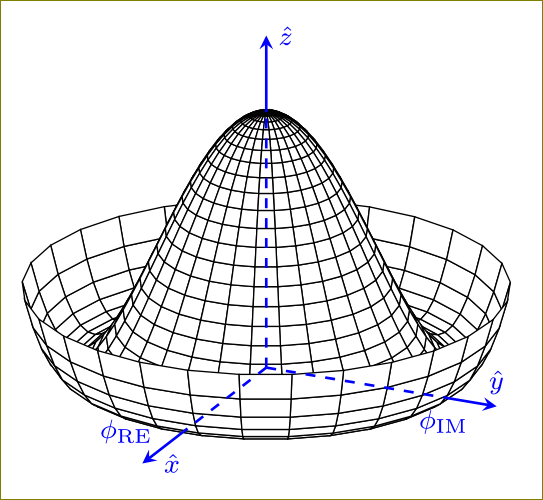
\includegraphics[width=0.4\linewidth]{figures/theory/higgs_potential.png}
    \caption{ A lower dimensionality representation of the shape of the Higgs
Potential.  The central peak represents a $v = 0$ rotationally symmetric
unstable state, while the trough represents the infinite choices of minima that
can be selected upon the spontaneous breaking of symmetry.}
    \label{fig:higgs_potential}
  \end{center}
\end{figure}

Whatever you call it, this potential is significant in
that its minimum is not at $\boldsymbol{\Phi} = 0$ but instead is symmetric
around the origin thus defining an infinite number of states that minimize V.
The value of this minima can be calculated by taking the derivative of V with
respect to $\boldsymbol{\Phi}$ and setting it equal to $0$. This value, also
known as the vacuum expectation value (vev) has been found to be $v \equiv
\sqrt{-\mu^{2}/\lambda} = 246$ GeV. In order to reach this ground state energy,
the Higgs field must spontaneously break this symmetry, and thus aquire an
arbitrary single value.  For ease of calculation we orient our coordinate system
such that

\begin{equation}
\left\langle \boldsymbol{\Phi}(x) \right\rangle = \frac{1}{\sqrt{2}} \left(
\begin{matrix} 0 \\ v \end{matrix} \right)
\end{equation} 

Next we parameterize small perturbations around the minimum of the Higgs
potential as 

\begin{equation} \label{eq:higgs:broken_higgs}
\left\langle \boldsymbol{\Phi}(x) \right\rangle = \frac{1}{\sqrt{2}} \left(
\begin{matrix} 0 \\ v + h(x) \end{matrix} \right) \text{exp} \left(
i\frac{\tau^{i}}{2}\theta^{i}(x) \right)
\end{equation} 

Here the real scalar field $h(x)$ corresponds to radial perturbations of the
minima and while the three $\theta^{i}(x)$ are the Nambu-Goldstone fields with
values determined by your choice of gauge.  Choosing the unitary gauge of
$\theta^{i}(x) = 0$ and expanding the kinetic term of
\Cref{eq:higgs:lagrangian} around the vev we get

\begin{equation} \label{eq:higgs:boson_masses}
\mathcal{L}_{\text{Higgs},K} = \frac{g^{2}v^{2}}{8} \left(
(W_{\mu}^{-})^{\dagger}W^{-\mu} + (W_{\mu}^{+})^{\dagger}W^{+\mu} \right) +
\frac{1}{2} \left( \begin{matrix} W_{\mu}^{3\dagger} & B_{\mu}^{\dagger}
\end{matrix} \right) \boldsymbol{M}^{2} \left( \begin{matrix} W^{3\mu} \\ B^{\mu}
\end{matrix} \right) + \ldots 
\end{equation}

Here the first term is the physical mass term for the $W^{\pm}$ bosons where we
have constructed their charge eigenstates ouf of the $W^{1,2}$ fields like this
$W^{\pm} = \frac{1}{\sqrt{2}}(W^{1} \mp iW^{2})$.  The second term represents the
mixture of the $W^{3}$ and $B$ fields through the mass matrix $\boldsymbol{M}$.
By diagonalizing this matrix and identifying the mass eigenstates we find the
physical fields of the photon ($\gamma$) and the $Z$ boson


\begin{equation}
\boldsymbol{M}_{Diagonalized}^{2} = \left( \begin{matrix} 0 & 0 \\ 0 &
\frac{v^{2}}{4}(g_{W}^{2} + g^{'2)}   \end{matrix} \right)
\end{equation}

The upper left diagonal element corresponds to the massless photon
while the lower right diagonal element gives the mass of the massive $Z$ boson.
This leaves us with the following masses for the 4 Electroweak bosons

\begin{equation}
m_{W} = \frac{1}{2}g_{W}v \quad , \quad m_Z = \frac{1}{2}v\sqrt{g_{W}^{2} + g^{'2}}
\quad , \quad m_\gamma = 0
\end{equation}

The masses of the $W^{\pm}$ and $Z$ gauge bosons can be related through the
Wineberg angle or mixing angle which

\begin{equation}
\theta_W = cos^{-1}\left( \frac{g_{W}}{\sqrt{g_{W}^{2}+g^{'2}}} \right) \rightarrow m_{Z} =
\frac{m_{W}}{cos{\theta_{W}}}
\end{equation}

Using this definition we can write out the exact mixture of $B$ and $W^{3}$ that
make up the photon and $Z$ boson

\begin{align}
\gamma &= \text{cos}(\theta_{W})B + \text{sin}(\theta_{W})W^{3} \\
Z &= -\text{sin}(\theta_{W})B + \text{cos}(\theta_{W})W^{3}
\end{align}

\subsection{Fermion Mass Terms} \label{sec:theory:fermion_mass}

In \Cref{sec:theory:qed} we saw that fermion mass terms violate gauge
invariance due to the mixing of the left and right chiral states.  The Higgs
mechanism again allows for a gauge invariant method of generating mass terms but
this time through the Yukawa coupling of the Higgs field to the fermion fields.
To see an example of this here is the Yukawa coupling term for the electron
doublet ($\boldsymbol{\Psi_L}$) and singlet ($\Psi_R$) coupling to the Higgs
field ($\boldsymbol{\Phi}$) after spontaneous symmetry breaking giving it the
form shown in \Cref{eq:higgs:broken_higgs} where we have again choosen
the unitary gauge $\Phi^{i}(x) = 0$.

\begin{align}
\mathcal{L}_{Yukawa} &= - g_{e} \left[ \boldsymbol{\bar{\Psi}_L}
\boldsymbol{\Phi} \Psi_R + \bar{\Psi}_{R} \boldsymbol{\Phi}^{\dagger} \boldsymbol{\Psi_L}
\right] \\ &= - \frac{g_{e}}{\sqrt{2}} \left[ \left( \begin{matrix}
\bar{\nu}_{e} & \bar{e} \end{matrix} \right)_L \left( \begin{matrix} 0 \\ \nu +
h \end{matrix} \right) e_{R} + \bar{e}_{R} \left( \begin{matrix} 0 & (\nu + h)
\end{matrix} \right) \left( \begin{matrix} \nu_{e} \\ e \end{matrix} \right)_L \ \right] \\ &= - \underbrace{\frac{g_{e}}{\sqrt{2}}
\nu}_{m_{e}} \left( \bar{e}_{L}e_{R} + \bar{e}_{R}e_{L}  \right)
- \underbrace{\frac{g_{e}}{\sqrt{2}}}_{g_{e,h}} h \left(
\bar{e}_{L}e_{R} + \bar{e}_{R}e_{L}  \right) 
\end{align}

And voila, we have successfully generated mass terms for our fermion field and
maintained the gauge invariance of our Lagrangian by using all gauge invariant
fields.  This operation has also left us with the second term which represents the coupling
of the elctron to the higgs itself thus giving us the form of it's coupling
constant $g_{e,h}$.  Using our newly found mass of the electron $m_{e}$ we can
write

\begin{equation}
g_{e,h} = \frac{g_{e}}{\sqrt{2}} = \frac{m_{e}}{\nu}
\end{equation}

Thus we see that the coupling of the higgs boson to a fermion is indeed
proportional to the mass of the fermion itself.  In other words, the more
massive a particle is, the more the higgs couples to it and vice versa.
 
\subsection{The Higgs Boson}

As we have seen this Higgs mechanism not only properly mixes the gauge fields
thus providing them gauge invariant mass terms, it also properly combines the
left and right chiral states of fermions to produce their mass terms.  The final
step then is to determine an observable of the theory that can be tested in
experiment, namely the existence of a massive scalar particle, the Higgs boson
intself.

Turning our attention to the potential term (V) of
\Cref{eq:higgs:lagrangian} and substituting in our definition for
$\boldsymbol{\Phi}$ given in \Cref{eq:higgs:broken_higgs} we find

\begin{equation}
\mathcal{L}_\text{Higgs,V} = \frac{1}{2} \mu^{2} \nu^{2} - \mu^{2} h^{2} +
\lambda \nu h^{3} + \frac{1}{4} \lambda h^{4}
\end{equation}

Here the first term is constant and thus can be ignored.  The second term is the
mass term for the SM particle the Higgs boson, $m_h = \sqrt{-2\mu^{2}} =
\sqrt{2\lambda}\nu$. Remembering that $h = h(x)$ was used for small radial
petrubrations of the Higgs field we can identify the Higgs boson simply as an
excitation of the Higgs field.  Finally, the third and fourth terms represent
the Higgs boson self-couplings.  With these couplings and mass terms in hand we
can now move on to the experimental verification of this theory as discussed
next in \Cref{chap:higgs}.

